\documentclass[12pt,a4paper]{report}
\usepackage[utf8]{inputenc}
\usepackage{amsfonts}
\usepackage{setspace}
\usepackage{graphicx}
\usepackage{array}
\usepackage{fancyhdr}
\usepackage{geometry}
\usepackage{ragged2e}
\usepackage{color}
\usepackage{biblatex}
\usepackage{tabularx}

\addbibresource{reference.bib}

\usepackage{color}
\geometry{
a4paper,
total={210mm,297mm},
left=1.0in,
right=0.85in,
top=0.65in,
bottom=0.65in,
}
\begin{document}
\pagestyle{empty}
\begin{center}

  {\large \textbf{Visvesvaraya Technological University, Belagavi – 590018}}
  \begin{figure}[hbtp]
    \centering
    
\includegraphics[width=2.3cm,height=3cm]{./pic/vtu}
  \end{figure}

  \textbf{PROJECT WORK DESIGN PHASE REPORT}
  \par
  \textbf{ON}
  \par
  \vspace{6pt}
  {\Large \textbf{Cloud-Based Smart Monitoring System for Baby Health and Safety}}
  \par
  \vspace{12pt}
  \par
  \textit{\textbf{Submitted in partial fulfillment of the requirements for the degree }}
  \par
  \vspace{12pt}
  \large \textbf{BACHELOR OF ENGINEERING }
  \par
  \textbf{in}
  \par
  \large \textbf{COMPUTER SCIENCE \& ENGINEERING}
  \par
  \vspace{12pt}
  \textit{\textbf{Submitted by}}
  \vspace{8pt}

  \begin{center}
    \begin{tabular}{l@{\hspace{2cm}}r}
      \textbf{\large Aaron Tauro}       & \textbf{4SO21CS002} \\
      \textbf{\large Abhik L Salian}    & \textbf{4SO21CS004} \\
      \textbf{\large Akhil Shetty M}    & \textbf{4SO21CS013} \\
      \textbf{\large H Karthik P Nayak} & \textbf{4SO21CS058} \\
    \end{tabular}
  \end{center}

  \vspace{12pt}
  \textit{\textbf{Under the Guidance of}}
  \par
  \vspace{6pt}
  \textbf{Dr Sridevi Saralaya}
  \par
  \vspace{2pt}
  \normalsize { Professor, Department of CSE }
  \par
  \begin{figure}[hbtp]
    \centering
    
\includegraphics[scale=0.6]{./pic/sjeclogo}
  \end{figure}
  \large \textbf{DEPT. OF COMPUTER SCIENCE AND ENGINEERING}
  \par \Large \textbf{ST JOSEPH ENGINEERING COLLEGE}
  \par
  \textbf{An Autonomous Institution}
  \par
  {\large{(Affiliated to VTU Belagavi, Recognized by AICTE, Accredited by NBA)}}
  \par
  \vspace{3pt}
  {\large \textbf{Vamanjoor, Mangaluru - 575028, Karnataka}}
  \par
  \vspace{12pt}
  {\Large \textbf{2024-25}}
\end{center}

\newpage

%%%%%%%%%%%%%%%%%%%%%%%%%% Acknowledgement %%%%%%%%%%%%%%%

% \pagestyle{empty}
% \setstretch{1.8}
% \pagenumbering{roman}
% \chapter*{\centering ACKNOWLEDGEMENT}


% The joy and satisfaction that accompany the partial completion of any task would be incomplete without thanking those who made it possible. We consider ourselves proud to be a part of St Joseph Engineering College, the institution which moulded us in all our endeavours. 
% We express our sincere gratitude to the management for providing state-of-the-art facilities and support throughout our project.
% \vspace{10pt}\\
% We owe our profound gratitude to our project guide \textbf{Dr Sridevi Saralaya}, Head of the Department, Computer Science and Engineering, St Joseph Engineering College, for her valuable guidance and support during the entire period of our project. 
% \vspace{10pt}\\
% We are indebted to our respected Principal, \textbf{Dr Rio D'Souza} for his valuable guidance and encouragement throughout the project.
% \vspace{10pt}\\
% We express our sincere gratitude to \textbf{Rev Fr Wilfred Prakash D'Souza}, Director, and \textbf{Rev Fr Kenneth Rayner Crasta}, Assistant Director, for their unwavering support and provision of facilities throughout the development stages of our project.
% \vspace{10pt}\\
% We wish to express our sincere gratitude to all the Faculty and Technical staff of the Department and friends and family for their valuable help and support during the period of development of our project .\\

\newpage

%%%%%%%%%%%%%%%%%%%%%%%%%% Abstract %%%%%%%%%%%%%%%
\pagestyle{empty}
\setstretch{1.5}

\chapter*{\centering ABSTRACT}

\begin{justify}
  Cloud-Based Smart Monitoring System for Baby Health and Safety is a software-driven solution designed to provide real-time monitoring and alerts for parents, focusing on the baby’s health and safety. The system collects data from various hardware sensors, including body temperature, room humidity, and heart rate, along with video feeds for continuous observation of the baby's movements. The software component plays a critical role by processing this data to detect abnormalities such as fever, unsafe sleeping postures (like tummy sleeping), and irregular movements, using cloud-based services and computer vision algorithms.

  \noindent A significant feature of the system is the streaming of the Raspberry Pi-based camera video data to the cloud, where the software analyzes the baby’s posture to help prevent risks such as Sudden Infant Death Syndrome (SIDS). The software also carries out detection of crying sounds, which triggers instant notifications to parents via the mobile application. The app also monitors environmental factors such as humidity and sends real-time alerts when unsafe conditions or health risks are detected. This phase of the project emphasizes the integration of cloud services, advanced data processing algorithms, and user-friendly notifications, ensuring robust, real-time monitoring with a focus on the software's efficiency.
\end{justify}

\setstretch{1.2}
\renewcommand{\contentsname}{\centering Table of Contents}
\tableofcontents

\newpage
\listoftables

\listoffigures








%%%%%%%%%%%%%%%%%%%%% Headders and Footers %%%%%%%%%%%%%%%
\fancyhf{} % clear header and footer
\fancyhead[L]{Bidirectional Communication System for Deaf-blind Individuals} % header centered
\fancyfoot[L]{Department of Computer Science and Engineering, SJEC, Mangaluru} % footer centered
\fancyfoot[R]{\thepage} % page number on the right
\renewcommand{\headrule}{%
  {\color[RGB]{97, 35, 34}\hrule width\headwidth height 2pt} % Top line
  \vspace{0.07\baselineskip}% Add space between lines
  {\color[RGB]{97, 35, 34}\hrule width\headwidth height 0.5pt} % Bottom line
}
\renewcommand{\footrule}{%

  {\color[RGB]{97, 35, 34}\hrule width\headwidth height 0.5pt} % Top line
  \vspace{0.07\baselineskip}% Add space between lines
  {\color[RGB]{97, 35, 34}\hrule width\headwidth height 2pt} % Bottom line
}


\renewcommand{\baselinestretch}{1.5}

% \pagestyle{fancy}
% \fancyhf{}
% \lhead{\fontsize{10}{12} \selectfont Bidirectional Communication System for Deaf-blind Individuals}
% \rhead{\fontsize{10}{12} \selectfont Chapter \thechapter}
% \lfoot{\fontsize{10}{12} \selectfont Department of Computer Science and Engineering, SJEC, Mangaluru}
% \rfoot{\fontsize{10}{12} \selectfont Page \thepage}
% \renewcommand{\headrulewidth}{0.5pt}
% \renewcommand{\footrulewidth}{0.5pt}


%%%%%%%%%%%%%%%%%%%%%%% CHapetr 1 Introduction %%%%%%%%%%%%%
\clearpage
\setcounter{page}{1}
\pagestyle{fancy}
\setstretch{1.2}
\pagenumbering{arabic}

\chapter{Introduction}
\par
\section{Background}
In contemporary society, communication serves as the cornerstone of human interaction, fostering connections, disseminating information, and enabling the exchange of ideas. However, for individuals confronting sensory impairments, particularly those who are both deaf and blind, these essential channels of communication become profoundly challenging to navigate. The deaf-blind community, often overlooked in technological advancements, faces formidable barriers to accessing and participating in text-based communication independently, thus exacerbating their isolation and limiting their ability to engage meaningfully with the world.

Despite remarkable strides in technology that have revolutionized communication for many, the unique challenges faced by the deaf-blind community persist. Traditional modes of communication, such as sign language and tactile sign language, while invaluable, often require face-to-face interaction or the presence of an interpreter. These limitations become increasingly pronounced in our digital age, where accessibility to efficient and portable communication solutions is paramount. As a consequence, the deaf-blind community remains largely excluded from the benefits of the digital world, hindering their capacity to connect with others, access information, and engage in everyday conversations.

Recognizing this significant gap in accessibility, our project proposes the development of a Multimodal Communication System specifically tailored to the needs of individuals who are both deaf and blind. This transformative initiative aims to empower the deaf-blind community by providing them with a means to engage effectively in text-based conversations, bridging the communication gap and enhancing their ability to connect with the world. The project's genesis lies in a commitment to inclusivity and the belief that technological innovation can serve as a powerful equalizer. By addressing the communication challenges faced by the deaf-blind community, we aspire to foster a more inclusive society where everyone, regardless of their abilities, can actively participate in the digital age. The subsequent sections outline the scope, methodology, and feasibility considerations of our project, providing a comprehensive roadmap for the development of a solution that promises to make a tangible impact on the lives of deaf-blind individuals.

\section{Problem statement }
To develop a specialized communication application tailored to meet the unique needs of individuals who are simultaneously deaf and blind, empowering them to engage effectively with the world and connect with others. Traditional methods of communication, such as sign language and tactile sign language, provide valuable means of interaction for the deaf-blind. However, these methods are often limited in scope, requiring face-to-face interaction or the physical presence of an interpreter. In an increasingly digital and mobile world, the lack of an efficient and portable solution for communication leaves the deaf-blind community at a significant disadvantage.


\section{Scope}
\textbf{Education:}
The system can be integrated into educational settings, allowing
deaf-blind students to participate in classroom discussions, access digital
educational materials, and communicate with teachers and peers.\\

\noindent\textbf{Personal Communication:}
The primary application is enabling deaf-blind
individuals to engage in text-based personal communication with their friends,
family, and colleagues. This can include text messages, emails, and social
media interactions.

%---------------------------- Chapter TWO --------------------------

\chapter{Literature Survey}

\section{MyVox-Device for the Communication Between People: Blind, Deaf, Deaf-Blind and Unimpaired}

The paper\cite{ref1} describes the development of the MyVox device, a communication system designed for individuals who are deaf-blind. The device is powered by an ARM-based computer, specifically the Raspberry Pi, and includes a USB keyboard for input, a speaker for speech synthesis, a braille display, a vibration motor for notifications, and a real-time clock for time perception.

The inputs of the device include a USB keyboard for text input, which can be customized to suit the user's needs, and the system also incorporates a real-time clock for time perception. The outputs of the device consist of an LCD display for text output, a speaker for speech synthesis, a braille refreshable display for tactile output, and a vibration motor for notifications. These components enable the device to provide communication capabilities for individuals who are deaf-blind, catering to their specific sensory needs and facilitating interaction with others.

The paper concludes by discussing future work, including the potential for internet access and custom applications, as well as plans to make the device available to more people in need. Overall, the MyVox device represents an important step forward in addressing the communication challenges faced by deaf-blind individuals and promoting social inclusion.

\section{Mobile Lorm Glove - Introducing a Communication Device for Deaf-Blind People }
The paper\cite{ref2} introduces the Mobile Lorm Glove, a communication device designed to support deaf-blind people's communication and enhance their independence.
The hardware prototype of the Mobile Lorm Glove includes fabric pressure sensors, vibrating motors, an ATmega328 microcontroller, shift registers, darlington transistor arrays, and a Bluetooth module for data transmission. The actuators on the glove are placed at varied distances to adjust stimulus duration, catering to individual tactile sensitivity and lorming speed. This customization allows for the adjustment of the maximal applied intensity and lorming speed to serve the user's needs.

The application scenarios for the Mobile Lorm Glove include mobile communication over distance and simultaneous translation. The glove enables the composition of text messages and their transmission to a receiver's handheld device, where the message can be read directly or translated into the Lorm alphabet using the Mobile Lorm Glove. Additionally, the glove functions as a simultaneous translator, allowing communication with individuals who are not familiar with Lorm, thus broadening the spectrum of people with whom deaf-blind individuals can engage. The device also enables parallel one-to-many communication, which can be particularly helpful in educational and learning contexts.

The Mobile Lorm Glove's input unit consists of fabric pressure sensors on the palm and a rectangular sensor on the wrist, which detect tactile input from the user's hand. These sensors transmit data to a microcontroller using a matrix design. The output unit comprises vibrating motors on the back of the glove, which provide haptic feedback based on the input received. The control unit, integrated with the microcontroller and a Bluetooth module, manages the data transmission between the glove and the user's handheld device. The user composes text messages by lorming onto their own left hand with the glove, and the data is transmitted to the handheld device for further processing or translation.

\section{Tactile Board: A Multimodal Augmentative and Alternative Communication Device for Individuals with Deafblindness}
The Tactile Board, a mobile Augmentative and Alternative Communication (AAC) device, is introduced as a groundbreaking solution to communication challenges faced by individuals with deafblindness\cite{ref3}. Characterized by dual sensory loss, deafblind individuals encounter difficulties compensating for impaired sight and hearing. The Tactile Board translates text and speech into real-time vibrotactile signs displayed through a haptic wearable, enabling deafblind individuals to communicate without direct assistance.

Based on interviews with 60 individuals with deafblindness across Europe, the Tactile Board features a 4-by-4 haptic matrix, customizable vocabulary database, and a haptic vest with coin-vibration motors. This facilitates two-way communication, addressing barriers to social interactions within the deafblind community. The paper underscores the limitations of existing technologies in meeting the unique challenges posed by dual sensory impairment, positioning the Tactile Board as a promising advancement in assistive technology.

The device's potential applications include communication with strangers, conveying environmental information, and supporting interactions in scenarios where direct touch is impractical, particularly relevant during the COVID-19 pandemic. The paper envisions future evaluations to assess the Tactile Board's impact on the confidence of individuals with deafblindness in initiating social interactions, contributing significantly to assistive technology for the deafblind community.
The Tactile Board employs a Samsung Galaxy Tab S2 tablet, Android OS, and Google's NLP API for speech recognition. RealTime Framework facilitates communication, while a Raspberry Pi and Python script translate data to on-off commands for coin-vibration motors in a haptic vest. The system incorporates 3D-printed cases and tactile tablet covers for accessibility.


\section{An Efficient Communication System for Blind, Dumb and Deaf People }
The paper\cite{ref4} outlines a project aimed at enhancing the lives of the blind, deaf, and dumb population in India, which comprises around 70 million people. The proposed system focuses on facilitating communication through sign language recognition, utilizing hand gestures for interaction between humans and computers. The system involves recording a user's voice, converting it to text on a server, classifying the text, generating corresponding signs, and transmitting them to applications for deaf or dumb individuals. Additionally, a reverse system for sign-to-speech communication is envisioned for visually impaired people. The background study references related work in object modeling, sign language character recognition, and American Sign Language translation through image processing. Technologies to be used include Blob Detection, Template Matching, and Skin Color Detection. The proposed system's characteristics include video initiation, hand sign recognition, a graphical user interface (GUI), and the ability to operate windows based on recognized signs. The system architecture involves a server for text conversion and sign generation, promoting efficient communication for the visually and hearing impaired. The conclusion emphasizes the system's potential to bridge communication gaps through image processing, enabling the recognition, storage, and use of sign language for various computer operations.

The proposed system for enhancing communication among the blind, deaf, and dumb in India utilizes image processing techniques. Technologies include Blob Detection, Template Matching, and Skin Color Detection. The system incorporates algorithms for recognizing hand signs, translating speech to text, and generating corresponding signs for improved interaction through sign language.
\section{Multimodal Communication System for People Who Are Deaf or Have Low Vision }
The paper\cite{ref5} addresses communication challenges confronting individuals with deafness or low vision, particularly concerning standard consumer products. Profoundly deaf individuals predominantly rely on text and graphics, lacking access to verbal communication channels like radio and television. The elderly, commonly affected by visual impairment, further complicates communication, and additional disabilities can exacerbate these challenges. The research aims to develop an inexpensive real-time transformation method for verbal messages to assist the profoundly deaf and visually impaired, emphasizing the necessity for a solution with minimal visual resource requirements.

The proposed system involves transforming textual information into visual color patterns, utilizing color tagging, Morse code, and the Phonetic Alphabet for temporal coding. The design incorporates light sources, such as LEDs, with brightness modulation for improved text visualization. The limitations of Morse code for real-time communication are discussed, prompting the suggestion of a single LED coupled with glasses to enhance direct viewing. This approach aims to improve text translation and perception for the deaf and visually impaired compared to traditional codes.

In conclusion, the novel light code variant, offering enhanced dynamic perception, holds potential benefits for the deaf, visually impaired, and as a peripheral display for wearable computer applications. The proposed approach demonstrates promise in advancing communication and visual perception for diverse user groups.

\section{A Communication System for Deaf and Dumb People }
The paper\cite{ref6} addresses communication challenges for deaf and mute individuals, highlighting speech's significance. Sign language, their primary form of communication, limits interaction with the outer world. Technology, particularly hand gesture recognition within human-computer interaction (HCI), is identified as a potential solution. An "artificial speaking mouth" concept is introduced, converting captured hand gestures into speech. This innovative technique could empower mute individuals to convey thoughts naturally. The literature survey underscores the communication disadvantage faced by mute individuals compared to blind counterparts using traditional language. A proposed solution involves dumb communication interpreters, translating hand gestures into speech. Flex Sensors in a digital glove facilitate sign language translation into speech, fostering communication between mute communities and the public.

The paper introduces a real-time hand gesture recognition system for HCI, utilizing the Kinect sensor. It outlines three modules: real-time hand tracking, training gestures, and gesture recognition using hidden Markov models. Challenges in recognizing small, complex hand articulations are acknowledged, proposing Kinect for improved human-computer interaction. The proposed system aims to bridge communication gaps for speech and hearing-impaired individuals, focusing on offline recognition through four processes: Image Acquisition, Preprocessing, Feature Extraction, and Classification. Proper segmentation, feature extraction, and classification are highlighted for successful recognition, reducing data dimensionality. The procedure, implemented and tested with 26 hand gesture images, plays gesture audio files upon recognition, enabling two-way communication and enhancing speech-hearing impaired individuals' communication capabilities.

\section{On Improving GlovePi: Towards a Many-to-Many Communication Among Deaf-blind Users }
The paper \cite{ref7} introduces an enhanced version of GlovePi, a low-cost wearable device designed to facilitate communication for deaf-blind individuals. The authors emphasize the significance of assistive technologies in promoting the inclusion, integration, and independence of people with disabilities, particularly those with deaf-blindness. The proposed extension of GlovePi's architecture aims to enable many-to-many communication, addressing the need for enhanced social interaction and daily activities for deaf-blind users. By focusing on improving communication capabilities, the authors aim to enhance the overall quality of life for deaf-blind individuals. The proposed enhancements in GlovePi demonstrate a commitment to leveraging technology to address the unique communication challenges faced by individuals with deaf-blindness, ultimately contributing to their social inclusion and well-being.

\section{HaptiComm: A Touch-Mediated Communication Device for Deafblind Individuals }
The paper\cite{ref8} presents HaptiComm, a touch-mediated communication device designed to facilitate communication for Deafblind individuals. The device uses an array of electrodynamic actuators to reproduce tactile sensations of fingerspelling, allowing for communication through touch. The paper describes the design and implementation of the device, including the actuator guidance system, which was developed to cancel magnetic interference between close actuators and keep the intended skin contacts. The study evaluated the device's ability to reproduce tactile sensations of fingerspelling and the participants' ability to recognize the type and number of activated actuators. The results showed that the device was able to reproduce three of the five contact types of fingerspelling, and that participants were able to accurately recognize the type and number of activated actuators. The authors suggest that HaptiComm has the potential to improve communication for Deafblind individuals and that further investigations are needed to explore its full potential. They plan to refine the timing and speed parameters of actuation and estimate the device's individual and sequenced letter recognition rate compared to human fingerspelling. They also plan to quantify the learning curve of the device, which is an essential element in the adoption of assistive technology.

Overall, the paper presents an innovative device that has the potential to improve communication for Deafblind individuals. The study provides valuable insights into the development and evaluation of HaptiComm, highlighting its strengths and limitations and suggesting avenues for future research.

\section{Proposed system}

\textbf{PLEASE NOTE: REMOVE THE QUESTION  AND WRITE ONLY THE ANSWERS \\}
\textbf{Why the Chosen Problem/Project is Important:} \\
The proposed Bidirectional Communication System for Deaf-Blind Individuals is of paramount importance as it addresses a critical and often overlooked issue, aiming to break down communication barriers and foster inclusivity. By providing a tailored solution for individuals who are both deaf and blind, the project empowers this community to actively engage in text-based communication, educational activities, and personal interactions. The system's integration in educational settings ensures equal opportunities for deaf-blind students, enabling their participation in classroom discussions and access to digital educational materials. Beyond education, the project promotes social connection by facilitating text-based communication through various channels. Moreover, it contributes to technological advancements for accessibility, reflecting a human-centric approach that recognizes and responds to the specific needs of the deaf-blind community. In essence, the project embodies the ethical responsibility of the technological community to create inclusive solutions, ultimately improving the quality of life for individuals facing unique challenges. \\



\noindent
\textbf{What is Novel in Proposed Project Work:} \\
The proposed project distinguishes itself through a novel integration of speech-to-text conversion and braille representation, providing a multimodal communication system for deaf-blind individuals. Notably, it addresses the educational context, empowering deaf-blind students to actively engage in classroom activities and digital learning. The inclusion of real-time braille hardware interaction, an intuitive user interface designed for the unique needs of deaf-blind users, and human-centric usability testing further set this project apart. By combining these elements, the project contributes to inclusive technological innovation, emphasizing accessibility and usability to enhance the communication experience for the deaf-blind community. \\

\noindent
\textbf{How it Would Advance the State-of-the-Art:} \\
The proposed project would advance the state-of-the-art by pioneering a multimodal communication system for deaf-blind individuals, seamlessly integrating speech-to-text conversion with real-time braille hardware interaction. Its focus on educational integration and an intuitive user interface tailored to the unique needs of deaf-blind users represents a groundbreaking contribution to inclusive education and user-centered design. The project's emphasis on human-centric usability testing ensures that technological advancements align with the practical needs and preferences of the deaf-blind community, setting a new standard in assistive technology for those with combined auditory and visual impairments. Overall, the project's comprehensive approach positions it at the forefront of innovative and inclusive communication solutions, advancing the current state-of-the-art in assistive technology. \\

\noindent
\textbf{How it Differs from Existing Works:} \\
Unlike existing solutions that often focus on singular aspects of communication for the deaf-blind, the proposed project innovates through its multimodal approach, seamlessly combining speech-to-text conversion with real-time interaction with dedicated braille hardware. Its unique emphasis on educational integration, user interface tailored for the deaf-blind, and human-centric usability testing further distinguish it. The project's comprehensive communication solution, covering various facets of accessibility, sets it apart from current works, marking a pioneering advancement in assistive technology for individuals with combined auditory and visual impairments..
\section{Comparison of existing methods}
In Table 2.1, we've laid out a comparison of different research studies. We're taking a close look at how each study has approached its work, what methods they've used to put their ideas into action, the conclusions they've come to, and the results they've achieved. We're also noting down the challenges each study has faced.

\begin{table}[h]
  \centering
  \caption{Comparison of Existing Projects}
  \renewcommand{\arraystretch}{1.5}
  \resizebox{\textwidth}{!}{
    \begin{tabular}{|>{\centering\arraybackslash}p{3.3cm}|>
      {\centering\arraybackslash}p{4.5cm}|>{\centering\arraybackslash}p{4.5cm}|>{\centering\arraybackslash}p{4.5cm}|>{\centering\arraybackslash}p{4.5cm}|>{\centering\arraybackslash}p{4.5cm}|}

      \hline

      \textbf{Project Title}                                                                                                           & \textbf{Problem Addressed}                                                                                             & \textbf{Methodology}                                                                                                                                                                   & \textbf{Implementation and Results}                                                                                                                     & \textbf{Inference and Results}                                                                                                                                                           & \textbf{Limitation/Future Scope}                                                                                                                                \\
      \hline
      Mobile Lorm Glove-Introducing a Communication Device for Deaf-Blind People (February 2012)                                       & Communication challenges for deaf-blind individuals                                                                    & Uses fabric pressure sensors, vibrating motors, and a Bluetooth module for communication                                                                                               & Enables mobile communication, simultaneous translation, and one-to-many communication                                                                   & Enhances independence and communication for deaf-blind individuals                                                                                                                       & Thickness of the glove                                                                                                                                          \\
      \hline
      Tactile Board: A Multimodal Augmentative and Alternative Communication Device for Individuals with Deafblindness (November 2020) & Communication challenges for individuals with deafblindness using a mobile AAC device                                  & Utilizes a 4-by-4 haptic matrix, customizable vocabulary database, and a haptic vest                                                                                                   & Employs Samsung Galaxy Tab S2, Android OS, Google's NLP API, Raspberry Pi, and Python script                                                            & Potential applications include communication with strangers and conveying environmental information.                                                                                     & Future evaluations are envisioned, especially during the COVID-19 pandemic                                                                                      \\
      \hline
      Multimodal Communication System for People Who Are Deaf or Have Low Vision (January 2002)                                        & Communication challenges for individuals with deafness or low vision                                                   & Involves real-time transformation of verbal messages into visual color patterns                                                                                                        & Uses LEDs with brightness modulation for improved text visualization.                                                                                   & Shows promise for real-time communication for individuals with hearing and vision impairments                                                                                            & Acknowledges limitations of Morse code and proposes a novel light code variant.
      \\
      \hline
      On Improving GlovePi: Towards a Many-to-Many Communication Among Deaf-blind Users (January 2018)                                 & Communication challenges for deaf-blind individuals, emphasizing many-to-many communication                            & Enhanced version of GlovePi with sensors, Raspberry Pi, mobile devices, and a tuple center                                                                                             & Focuses on improving communication capabilities for enhanced social interaction                                                                         & Aims to contribute to the social inclusion and well-being of deaf-blind individuals                                                                                                      & Future work involves integrating output sensors for tactile feedback.                                                                                           \\
      \hline
      MyVox-Device for the Communication Between People: Blind, Deaf, Deaf-Blind and Unimpaired (October 2014)                         & Developed for individuals who are deaf-blind, addressing their communication challenges                                & Powered by Raspberry Pi, includes USB keyboard, speaker, braille display, vibration motor, and real-time clock                                                                         & Provides customized inputs and outputs for text, speech, and tactile communication                                                                      & Represents an important step in addressing the communication challenges faced by deaf-blind individuals                                                                                  & Future work involves internet access, custom applications, and broader availability                                                                             \\
      \hline
      HaptiComm: A Touch-Mediated Communication Device for Deafblind Individuals (April 2023)                                          & Communication challenges for Deafblind individuals through touch-mediated communication using electrodynamic actuators & Utilizes an array of electrodynamic actuators to reproduce tactile sensations of fingerspelling, with a focus on canceling magnetic interference and addressing shaking and vibrations & Successfully reproduces three of the five contact types of fingerspelling, participants accurately recognize the type and number of activated actuators & Further investigations are needed to explore its full potential, including refining timing and speed parameters and estimating letter recognition rates compared to human fingerspelling & Acknowledges susceptibility to shaking and vibrations, plans to refine actuation parameters, estimate letter recognition rates, and quantify the learning curve \\
      \hline
    \end{tabular}
  }
  \label{tab:gesture-recognition-projects}
\end{table}



\chapter{Software Requirements Specification}
\section{Functional requirements}

\textbf{Speech-to-Text Conversion:}\\
Integrate robust speech recognition tools or APIs, such as Google Cloud Speech-to-Text or Python's SpeechRecognition library. Capture and transcribe spoken words into written text. Ensure high accuracy in speech-to-text conversion to facilitate precise communication.

\noindent\textbf{Text-to-Braille Conversion:}\\
Develop a sophisticated algorithm capable of translating transcribed text into Braille characters. Support different Braille standards and languages. Efficiency to minimize processing time for text-to-Braille conversion.

\noindent\textbf{Braille Hardware Integration:}\\
Integrate with Braille hardware systems i.e. device containing the sensor and actuators. Enable real-time sensory updates for seamless interaction.

\noindent\textbf{User Interface Development:}\\
Design an intuitive user interface for easy interaction.
Facilitate smooth communication between the application and Braille hardware.

\noindent\textbf{Hardware Interaction:}\\
Develop a system that interfaces seamlessly with the chosen Braille hardware.
Ensure the application can send Braille characters to the hardware for physical representation.

\section{Non-Functional requirements}
\textbf{Security Measures:}\\
Implement robust security protocols to ensure user data privacy and secure communication.

\noindent\textbf{Usability Testing:}\\
Conduct extensive usability testing with deaf-blind users to evaluate system functionality. Gather feedback for continual improvement.

\noindent\textbf{Accessibility Standards Compliance:}\\
Ensure compliance with accessibility standards to cater to the specific needs of the deaf-blind community. Test and enhance the application's compatibility with different screen reader software.

\noindent\textbf{Language and Braille Standards Support:}\\
Support Braille standards to enhance versatility and stay updated with the latest Braille standards and ensure compatibility

\section{User Interface Designs}
\textbf{Intuitive Design:}\\
\qquad Simple Navigation:
Design a straightforward navigation system that is easy for deaf-blind users to comprehend. Utilize clear and concise menu structures to facilitate intuitive interaction.

\noindent\textbf{Accessibility Features:}\\
Tactile Feedback Options:
Integrate tactile feedback options within the user interface to enhance the user experience for deaf-blind individuals. Provide customizable settings for feedback intensity and type.

\noindent\textbf{Design specifications:}\\
Maintain a consistent design language across the website and application to provide a unified user experience. Design the website to be responsive across different devices, ensuring accessibility on desktops, tablets, and smartphones.


\section{Hardware and Software requirements}
\subsection{Hardware Requirements:}

\textbf{Sensors for Braille Input:}\\
Deploy sensors capable of detecting Braille characters either through touch or proximity sensors. Ensure the sensors are responsive to user input for a seamless interaction experience.

\noindent\textbf{Actuators for Tactile Feedback:}\\
Integrate actuators to provide tactile feedback corresponding to the Braille characters displayed. Design the actuators to deliver precise and distinguishable tactile sensations for each Braille character.

\noindent\textbf{Braille Symbol Actuator/Sensor:}\\
Employ a hardware system as the primary hardware interface. Ensure the device can dynamically represent different Braille characters based on user inputs and can sense.

\subsection{Software Requirements:}

\textbf{Speech-to-Text Conversion Software:}\\
Utilize reliable speech recognition tools such as APIs, PyAudio, SpeechRecognition, and librosa by Python library for accurate conversion of spoken words into written text. Select a technology stack that supports real-time speech-to-text conversion.

\noindent\textbf{Text-to-Braille Conversion Algorithm:}\\
Develop a robust algorithm for translating the transcribed text into Braille characters using Python. Ensure the algorithm supports various Braille standards and languages.

\noindent\textbf{Braille to Hardware Translation Software:}\\
Implement software to translate the Braille characters into signals that can be understood by the hardware. Developing a communication protocol using a hardware device that can be used by sensing for seamless interaction between the software and hardware components.

\noindent\textbf{Website or Application:}\\
Create a user-friendly website or application interface for text-based communication. Include features for speech-to-text conversion, text-to-Braille conversion, and seamless interaction with the hardware.

\noindent\textbf{Operating System Compatibility:}\\
Ensure compatibility with major operating systems, such as Android and iOS, for mobile applications. For websites, ensure compatibility across different web browsers.

\noindent\textbf{Integration with ROS (Robot Operating System):}\\
Implement the necessary software components to integrate with ROS. Ensure smooth communication between different software modules.


\section{Performance Requirements }
\textbf{Real-time Speech-to-Text Conversion:}\\
Achieve near-instantaneous speech-to-text conversion. Evaluate system response time for spoken words to text. Ensure real-time transcription for effective communication.

\noindent\textbf{Efficient Text-to-Braille Translation:}\\
Swift translation of text to Braille characters. Assess the speed of the text-to-Braille conversion algorithm. Minimize delays in Braille representation.

\noindent\textbf{Seamless Hardware Interaction:}\\
Establish real-time communication with Braille hardware. Monitor time for Braille characters to be transmitted and displayed. Achieve responsive updates on the Braille hardware.

\noindent\textbf{Scalability:}\\
Ensure optimal performance with increased user interactions. Evaluate system performance under varying loads. Maintain optimal performance with a growing user base and data load.

\noindent\textbf{Resource Utilization:}\\
Optimize resource usage for efficient operation. Assess CPU, memory, and network utilization. Ensure resource-efficient operation on diverse devices.

\noindent\textbf{Error Handling:}\\
Implement effective error-handling mechanisms. Evaluate the system's ability to manage errors. Gracefully handle errors to minimize disruption.

\noindent\textbf{Usability Testing:}\\
Conduct usability testing based on user feedback. Gather feedback on system responsiveness and ease of use. Regular testing and iterative improvements for user satisfaction.


\section{Design Constraints}
\textbf{Portability:}\\
The system must be designed for portability, considering use across different devices. Optimize the user interface and functionalities for seamless operation on various platforms, including mobile devices and desktop computers.

\noindent\textbf{Device Compatibility:}\\
Ensure compatibility with a variety of devices commonly used by the deaf-blind community. Design the system to adapt to different screen sizes, resolutions, and hardware configurations for widespread accessibility.

\noindent\textbf{Real-time Communication:}\\
Address the need for real-time communication between the application and hardware. Optimize data transmission and processing to minimize latency, providing users with immediate updates on the Braille hardware.

\noindent\textbf{Usability for Deaf-Blind Users:}\\
Prioritize usability for individuals with dual sensory impairments. Conduct usability testing with the deaf-blind community, incorporating their feedback to optimize the system's accessibility and ease of use.

\section{Other Requirements}
\textbf{Long-term Support Plans:}\\
Develop strategies for long-term system support and updates. Establish a framework for ongoing maintenance, addressing evolving technological standards and user needs.

\noindent\textbf{Training Programs:}\\
Provide comprehensive training programs for users, educators, and support staff. Design training materials and sessions to ensure effective usage and support, promoting accessibility and user empowerment.

% \chapter{System Design}
% \section{Abstract Design}
% \subsection{Architectural Diagram}

% \begin{figure}[hbtp]
% \centering

% 
\includegraphics[width=0.6\textwidth, height=0.7\textwidth]{./pic/sjeclogo.png}\\
% \caption{Architectural Diagram}
% \end{figure}

% \noindent This architectural diagram illustrates the interaction of modules like Speech-to-Text Conversion Module, Text-to-Braille Conversion Module, and Braille Hardware Integration Module in the User Interface Layer\\

% \noindent\textbf{User Interface Layer:}\\
% This layer includes the Speech-to-Text Conversion Module, Text-to-Braille Conversion Module, and Braille Hardware Integration Module. Users interact with the system through this layer, which provides various input options and tactile feedback.\\

% \noindent\textbf{Speech-to-Text Conversion Module:}\\
% The Speech-to-Text Conversion Module is a component of a system that converts spoken language (speech) into written text (text). It utilizes specific algorithms, techniques and tools to transcribe spoken words into textual form.\\

% \noindent\textbf{Text-to-Braille Conversion Module:}\\
% The Text-to-Braille Conversion Module is a component of a system that translates textual information into Braille characters. Braille is a tactile writing system used by people who are blind or visually impaired to read and write.\\

% \noindent\textbf{Braille Hardware Integration Module:}\\
% The Braille Hardware Integration Module is a component of a system that facilitates communication between the software or digital system and Braille hardware devices. It acts as a bridge, enabling the software to send information to the Braille hardware for tactile representation and receive sensory feedback from the hardware.\\

% \subsection{Use case Diagram}

% \begin{figure}[hbtp]
% \centering

% 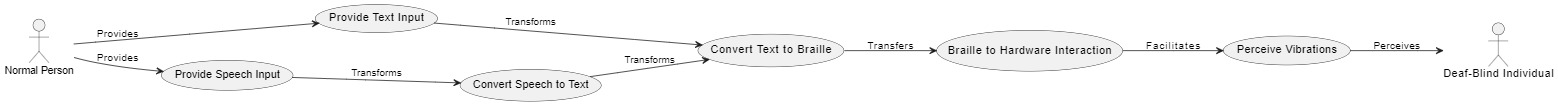
\includegraphics[width=1\textwidth, height=0.2\textwidth]{./pic/UC2.jpg}\\
% \caption{Use case Diagram}
% \end{figure}

% \noindent This use case diagram illustrates the interactions between actors and the system's functionalities in facilitating communication for the deaf-blind community, from input provision by a normal person to the ultimate perception of vibrations by a deaf-blind individual\\\\
% \noindent\textbf{Actors:}\\
% Normal Person: Represents individuals who interact with the system to provide input, either in the form of text or speech.\\
% Deaf-Blind Individual: Represents individuals who are the ultimate recipients of the communication facilitated by the system.\\

% \noindent\textbf{Use Cases:}\\
% Provide Text Input: Use case where the normal person provides input in the form of text to the system.
% \\Provide Speech Input: Use case where the normal person provides input in the form of speech to the system.
% \\Convert Speech to Text: Use case where the system converts the speech input provided by the normal person into text format.
% \\Convert Text to Braille: Use case where the system converts input, whether text provided directly or speech converted to text, into Braille format.
% \\Braille to Hardware Interaction: Use case where the system interacts with Braille hardware to convert Braille output into physical vibrations.
% \\Perceive Vibrations: Use case where the vibrations generated by the hardware are perceived by the deaf-blind individual, facilitating communication.\\

% \noindent\textbf{Actor-Use Case Relationships:}\\
%  Normal Person to Use Cases: The "Normal Person" actor interacts with the system by providing text or speech input, which triggers the corresponding use cases.
% \\Deaf-Blind Individual to Perceive Vibrations Use Case: The "Deaf-Blind Individual" actor perceives the vibrations generated by the hardware, which is represented by the "Perceive Vibrations" use case.\\


% \noindent\textbf{Use Case Relationships:}\\
% Convert Speech to Text to Convert Text to Braille: The "Convert Speech to Text" and "Convert Text to Braille" use cases are connected, indicating that the text output from speech conversion is further processed to convert it into Braille format.
% \\Text Input and Speech Input to Convert Text to Braille: Both "Provide Text Input" and "Provide Speech Input" use cases are connected to "Convert Text to Braille," indicating that regardless of the input method, the system converts it to Braille for further processing.




% \section{Functional Design}
% \subsection{Sequence Diagram}

% \begin{figure}[hbtp]
% \centering

% 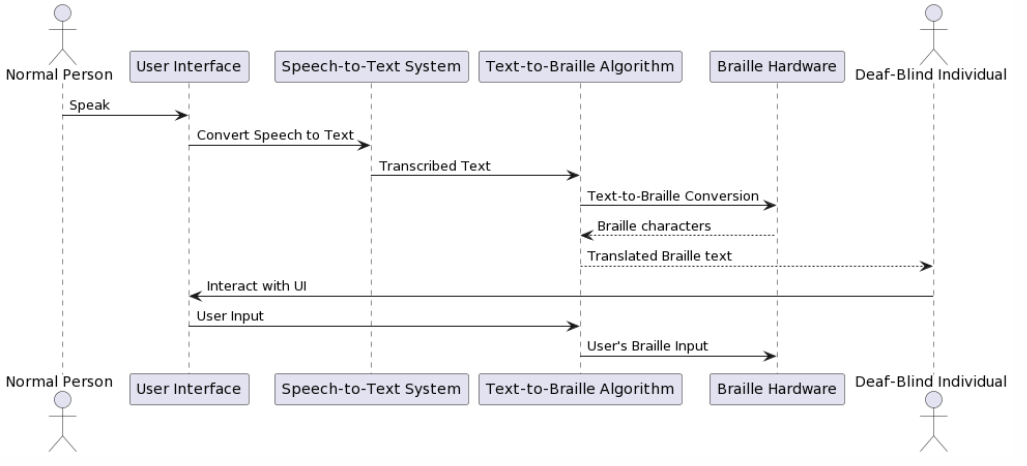
\includegraphics[width=1\textwidth, height=0.6\textwidth]{./pic/seq.png}\\
% \caption{Sequence Diagram}
% \end{figure}

% \noindent\textbf{Normal Person Interaction:}\\
% The communication process commences with the "Normal Person" initiating a conversation by speaking. This reflects the conventional method of conveying information, allowing for natural and spontaneous communication.

% \noindent\textbf{Speech-to-Text Conversion:}\\
% The spoken words are captured by the system's "User Interface," representing the first step in the conversion process. The "User Interface" serves as the gateway for the normal person to interact with the system.
% The speech is then processed by the "Speech-to-Text System," employing robust speech recognition tools or APIs such as Google Cloud Speech-to-Text or Python's SpeechRecognition library. This step ensures the accurate conversion of spoken words into written text.
% The accuracy of speech-to-text conversion is crucial for maintaining the fidelity of the communicated information, enabling precise and meaningful interactions between the normal person and the deaf-blind individual.\\

% \noindent\textbf{Text-to-Braille Conversion:}\\
% The transcribed text undergoes the next transformation through the "Text-to-Braille Algorithm." This sophisticated algorithm is designed to translate the transcribed text into Braille characters, catering to the specific needs of the deaf-blind individual.
% The algorithm supports various Braille standards and languages, ensuring versatility in communication. Additionally, efficiency is prioritized to minimize processing time for text-to-Braille conversion, facilitating a near real-time communication experience.
% This stage in the process is pivotal, as it bridges the gap between the digital representation of text and its tactile counterpart in the form of Braille. The system aims to provide a seamless and efficient means of communication for the deaf-blind individual.\\\\

% \noindent\textbf{Braille Hardware Integration:}\\
% The translated Braille characters are then transmitted to the "Braille Hardware," which constitutes a handheld device containing sensors and actuators. This integration allows for the physical representation of Braille characters, enabling the deaf-blind individual to read and understand the communicated information through tactile feedback.
% Real-time sensory updates from the Braille Hardware ensure a dynamic and responsive interaction experience. This stage emphasizes the tangible aspect of communication, recognizing the importance of tactile feedback for individuals who are both deaf and blind.\\

% \noindent\textbf{Communication to Deaf-Blind Individual:}\\
% The Braille Hardware communicates the translated Braille text directly to the "Deaf-Blind Individual," establishing a direct link between the information conveyed by the normal person and the tactile representation experienced by the deaf-blind individual.
% This direct communication channel ensures that the deaf-blind individual receives the information in a format that is accessible and meaningful, fostering effective communication and understanding.\\

% \noindent\textbf{User Interface Interaction:}\\
% Simultaneously, the deaf-blind individual has the opportunity to interact with the "User Interface." This interaction loop provides a means for the user to actively engage with the system beyond receiving information, contributing to a more participatory communication experience.
% The user interface serves as a central hub for user input, allowing the deaf-blind individual to provide feedback, respond to prompts, or initiate interactions. This bidirectional communication aspect enhances the inclusivity and versatility of the system.


% \section{Access Layer Design}
% \subsection{Dataflow Diagram}

% \begin{figure}[hbtp]
% \centering

% 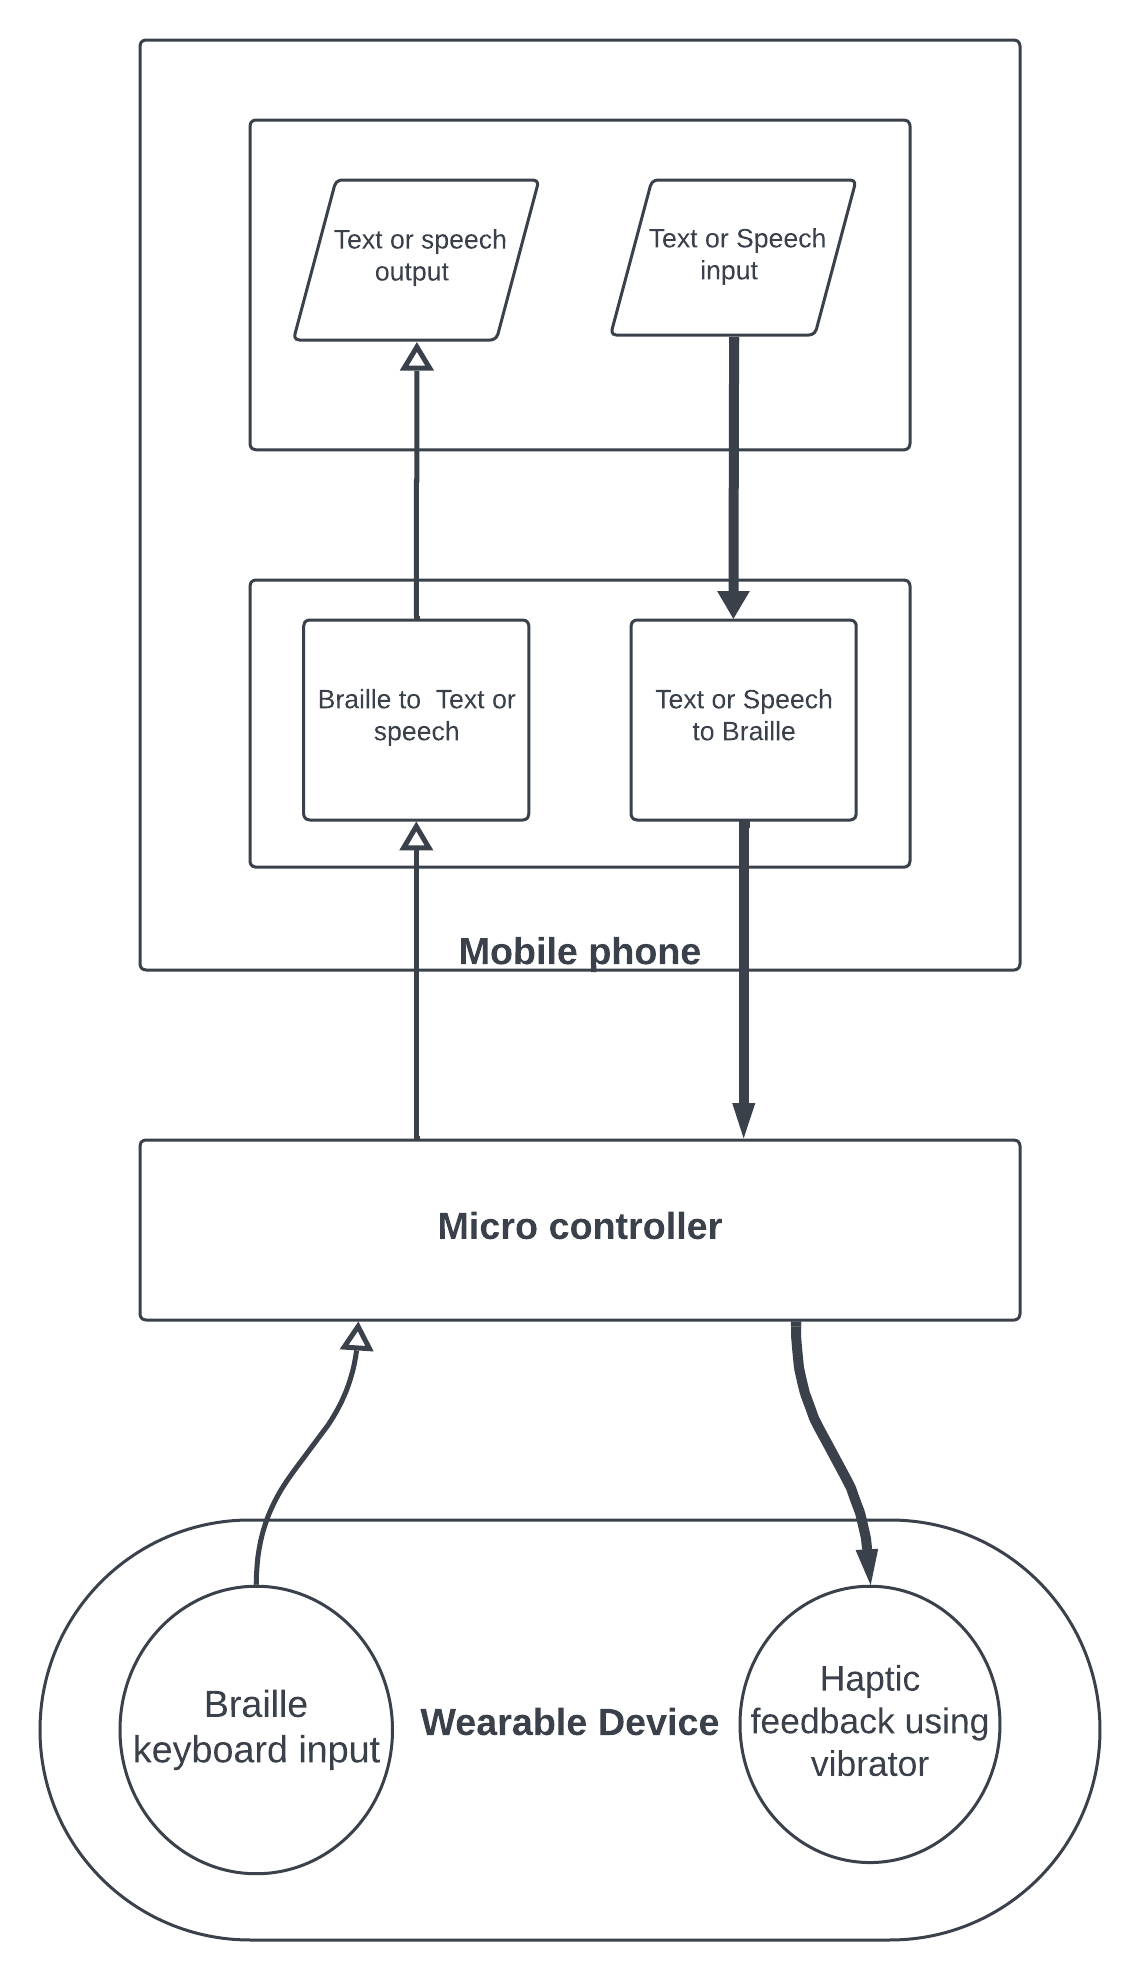
\includegraphics[width=0.7\textwidth, height=1\textwidth]{./pic/dataflow.png}\\
% \caption{Dataflow diagram}
% \end{figure}

% \noindent 
% A Data Flow Diagram (DFD) visually represents the pathway of data within a system, illustrating the flow from textual input by a typical user to haptic output for the deaf-blind individual. Additionally, it portrays the flow from braille input by the deaf-blind individual to textual output for the typical user.\\

% \noindent\textbf{Mobile phone:}\\
% The mobile phone serves as the central platform for executing the software components of the program. It facilitates various essential tasks, such as capturing user input in the form of text or speech, converting this input into braille for tactile feedback, and reciprocally, transforming braille input into textual or audible output. This multifaceted functionality encapsulates the core operations of the program, enabling seamless communication between users with diverse sensory capabilities.\\

% \noindent\textbf{Micro controller:}\\
% The microcontroller component of the system processes braille signals received from the user, interpreting them to activate the appropriate actuators for tactile feedback. Additionally, it collects input from the deaf-blind individual, facilitating communication by sending this data to the mobile phone for processing and interpretation.\\ This microcontroller-mediated exchange ensures efficient interaction between the user and the system, enhancing accessibility for individuals with sensory impairments.\\

% \noindent\textbf{Wearable device:}\\
% The wearable device serves as the primary interface for the deaf-blind individual to interpret incoming braille signals from the phone. Positioned on the palm of the user, it features three actuators on each hand, representing the six dots of braille. These actuators provide tactile feedback, enabling the user to perceive the braille characters through touch.\\
% Beyond tactile feedback, the wearable device also facilitates communication by collecting inputs from the deaf-blind individual. These inputs are then transmitted to the mobile phone for processing and further interaction with the typical user. By bridging the communication gap between the deaf-blind individual and the broader user community, the wearable device enhances accessibility and facilitates meaningful interactions for individuals with sensory impairments.

\chapter{System Design}
paragraph contents...
\section{Architecture Design}
\begin{figure}[hbtp]
  \centering
  
\includegraphics[width=4in,height=3in]{./pic/sjeclogo.png}
  \caption{System Architecture Diagram}
  \label{fig:1}
\end{figure}
This Figure \ref{fig:1} illustrates a high-level overview of the audio visual speech separation system. It is important to note that the specific techniques, algorithms, and models used in each component can vary depending on the implementation approach and the requirements of the system.
\section{Complete system flow diagram}
\begin{figure}[hbtp]
  \centering
  
\includegraphics[width=5in,height=3in]{./pic/sjeclogo.png}
  \caption{Complete system flow diagram}
  \label{fig:2}
\end{figure}
\newpage
Figure \ref{fig:2}represent the flow chart of the proposed system. In audio visual speech separation, the goal is to decompose an audio signal containing multiple overlapping speakers into individual speech signals corresponding to each speaker. The decomposition process involves separating the desired speech signals from the background noise and other interfering sounds.

\section{Sequence diagram}
\par
The audio input undergoes pre-processing, while the visual input is processed to extract relevant cues. The pre-processed audio and processed visual data are then integrated. From the integrated representation, features are extracted. These features are utilized in the speech separation stage, where individual speech signals are separated from the mixture. Post-processing techniques are applied to enhance the quality of the separated speech signals. Finally, the individual speech signals are outputted as the result of the system. The sequence diagram shown in \ref{fig:3} ensures a sequential flow of operations, starting from capturing and processing the inputs, integrating the audio-visual information, extracting features, performing speech separation, applying post-processing, and generating the output. This design allows for effective processing and separation of audio visual data to obtain distinct speech signals from overlapping speakers.
\\
\begin{figure}[hbtp]
  \centering
  
\includegraphics[width=4in,height=2in]{./pic/sjeclogo.png}
  \caption{Sequence diagram}
  \label{fig:3}
\end{figure}



\newpage
\section{Use case Diagram}
Use cases represent the main functionalities and tasks involved in the audio visual speech separation system. Each use case contributes to the overall process of capturing, processing, integrating, separating, and post-processing the audio and visual data to achieve the desired outcome of individual speech signal separation as shown in Figure \ref{fig:4}.
\begin{description}
  \item [Pre-process Audio:] This use case involves pre-processing the captured audio data. It may include operations like filtering, noise reduction, and echo cancellation to improve the quality of the audio signals.

  \item [Process Visual:] This use case involves processing the captured visual data. It includes tasks such as face detection, facial landmark tracking, or lip motion analysis to extract relevant visual cues associated with speech production.

  \item [Integrate Audio-Visual:] This use case represents the integration of the pre-processed audio data and processed visual data to create a synchronized audio-visual representation, aligning the audio and visual streams.
\end{description}

\begin{figure}[hbtp]
  \centering
  
\includegraphics[width=2in,height=2in]{./pic/sjeclogo.png}
  \caption{Use case diagram for customer}
  \label{fig:4}
\end{figure}




\newpage
\renewcommand{\bibname}{References}

\begin{thebibliography}{35}
  \addcontentsline{toc}{chapter}{References}
  \bibitem{ref1}
  Ramirez-Garibay, F., Olivarria, C. M., Eufracio Aguilera, A. F., and Huegel, J. C. (2014). MyVox—Device for the communication between people: blind, deaf, deaf-blind and unimpaired. IEEE Global Humanitarian Technology Conference (GHTC 2014), 12, 506–509. https://doi.org/10.1109/ghtc.2014.6970330


  \bibitem{ref2}
  Ulrike Gollner, Tom Bieling, and Gesche Joost. 2012. Mobile Lorm Glove: introducing a communication device for deaf-blind people. In Proceedings of the Sixth International Conference on Tangible, Embedded and Embodied Interaction (TEI '12). Association for Computing Machinery, New York, NY, USA, 127–130. https://doi.org/10.1145/2148131.2148159

  \bibitem{ref3}
  Arthur Theil, Lea Buchweitz, James Gay, Eva Lindell, Li Guo, Nils-Krister Persson, and Oliver Korn. 2020. Tactile Board: A Multimodal Augmentative and Alternative Communication Device for Individuals with Deafblindness. In Proceedings of the 19th International Conference on Mobile and Ubiquitous Multimedia (MUM '20). Association for Computing Machinery, New York, NY, USA, 223–228. https://doi.org/10.1145/3428361.3428465

  \bibitem{ref4}
  Narute, P., Pote, A., Poman, A., and Pawar, S. (2018). An efficient communication system for blind, dumb and deaf people. International Research Journal of Engineering and Technology (IRJET), 5(1), 1561-1563.

  \bibitem{ref5}
  Evreinova, T., Evreinov, G., and Raisamo, R. (2002). Communication system for the people who are deaf or have low vision. In Proceedings of HANDICAP 2002 2ème Conférence pour l'essor des technologies d'assistance (pp. 115-120)

  \bibitem{ref6}
  Ghorpade, S. R., and Waghmare, S. K. (2015). A Communication System for Deaf and Dumb People. Hand, 1, 2.

  \bibitem{ref7}
  Monti, L., and Delnevo, G. (2018). On improving GlovePi: Towards a many-to-many communication among deaf-blind users. 2018 15th IEEE Annual Consumer Communications \&amp; Networking Conference (CCNC), 9, 1–5. https://doi.org/10.1109/ccnc.2018.8319236

  \bibitem{ref8}
  Duvernoy, B., Kappassov, Z., Topp, S., Milroy, J., Xiao, S., Lacôte, I., Abdikarimov, A., Hayward, V., and Ziat, M. (2023). HaptiComm: A Touch-Mediated Communication Device for Deafblind Individuals. IEEE Robotics and Automation Letters, 8(4), 2014–2021. https://doi.org/10.1109/lra.2023.3241758023, doi: 10.1109/LRA.2023.3241758.
\end{thebibliography}
\end{document}